\documentclass[main.tex]{subfiles}

\begin{document}
\chapter{Central Results}
\lhead{Central Results}
\label{chap:results}

\section{English LUKE Reproduction}%
\label{sec:English LUKE Reproduction}
\begin{table}[H]
	\begin{center}
		\begin{tabular}{l c c c c c}
			Model & Micro avg. & LOC & PER & ORG & MISC \\
			\hline
			LUKE large & $94.00 \pm  0.2$ & $94.99 \pm  0.09$ & $97.19 \pm  0.1$ & $93.63 \pm  0.3$ & $85.29 \pm  1$ \\
			LUKE base & $93.42 \pm  0.2$ & $94.67 \pm  0.2$ & $96.89 \pm  0.2$ & $92.41 \pm  0.2$ & $84.94 \pm  0.7$ \\
			 &  &  &  &  &  \\
			Support & 5616 & 1666 & 1602 & 1647 & 701 \\
		\end{tabular}
	\end{center}
	\caption{Mean F1\pro\ scores and standard deviation over five repetitions of fine-tuning and evaluating LUKE on CoNLL2003 for each model size.}
%    TODO: If not already, it should be stated somewhere that all multiclass F1 refer to micro average
	\label{tab:lukeF1s}
\end{table}

\section{Pretraining of daLUKE}%
\label{sec:Pretraining of daLUKE}
\begin{enumerate}
    \item Resultater for maskerede opgaver
    \item Alle træningskurverne for hovedeksperimentet
\end{enumerate}

\begin{table}[H]
    \centering
    \begin{tabular}{l|rrrrrr}
        Top $k$ accuracy [\pro] & $k=1$  & $k=3$ & $k=5$ & $k=10$ & $k=25$ & $k=50$\\\hline
        Masked words            & 24.82       & 31.54      & 34.96      & 40.27       & 48.15       & 54.02      \\
        Masked entities         & 56.17       & 68.58      & 73.58      & 79.78       & 86.36       & 90.27
    \end{tabular}
    \caption{
        The main pretrained model performance in the last of 150 epochs.
        The measures are frequency of correct prediction on the two mask prediction tasks, when considering a prediction to be correct if the true token is one $K$ most likely labels according to the model softmax output.
    }
    \label{tab:mainpre}
\end{table}\noindent

\begin{figure}[H]
    \centering
    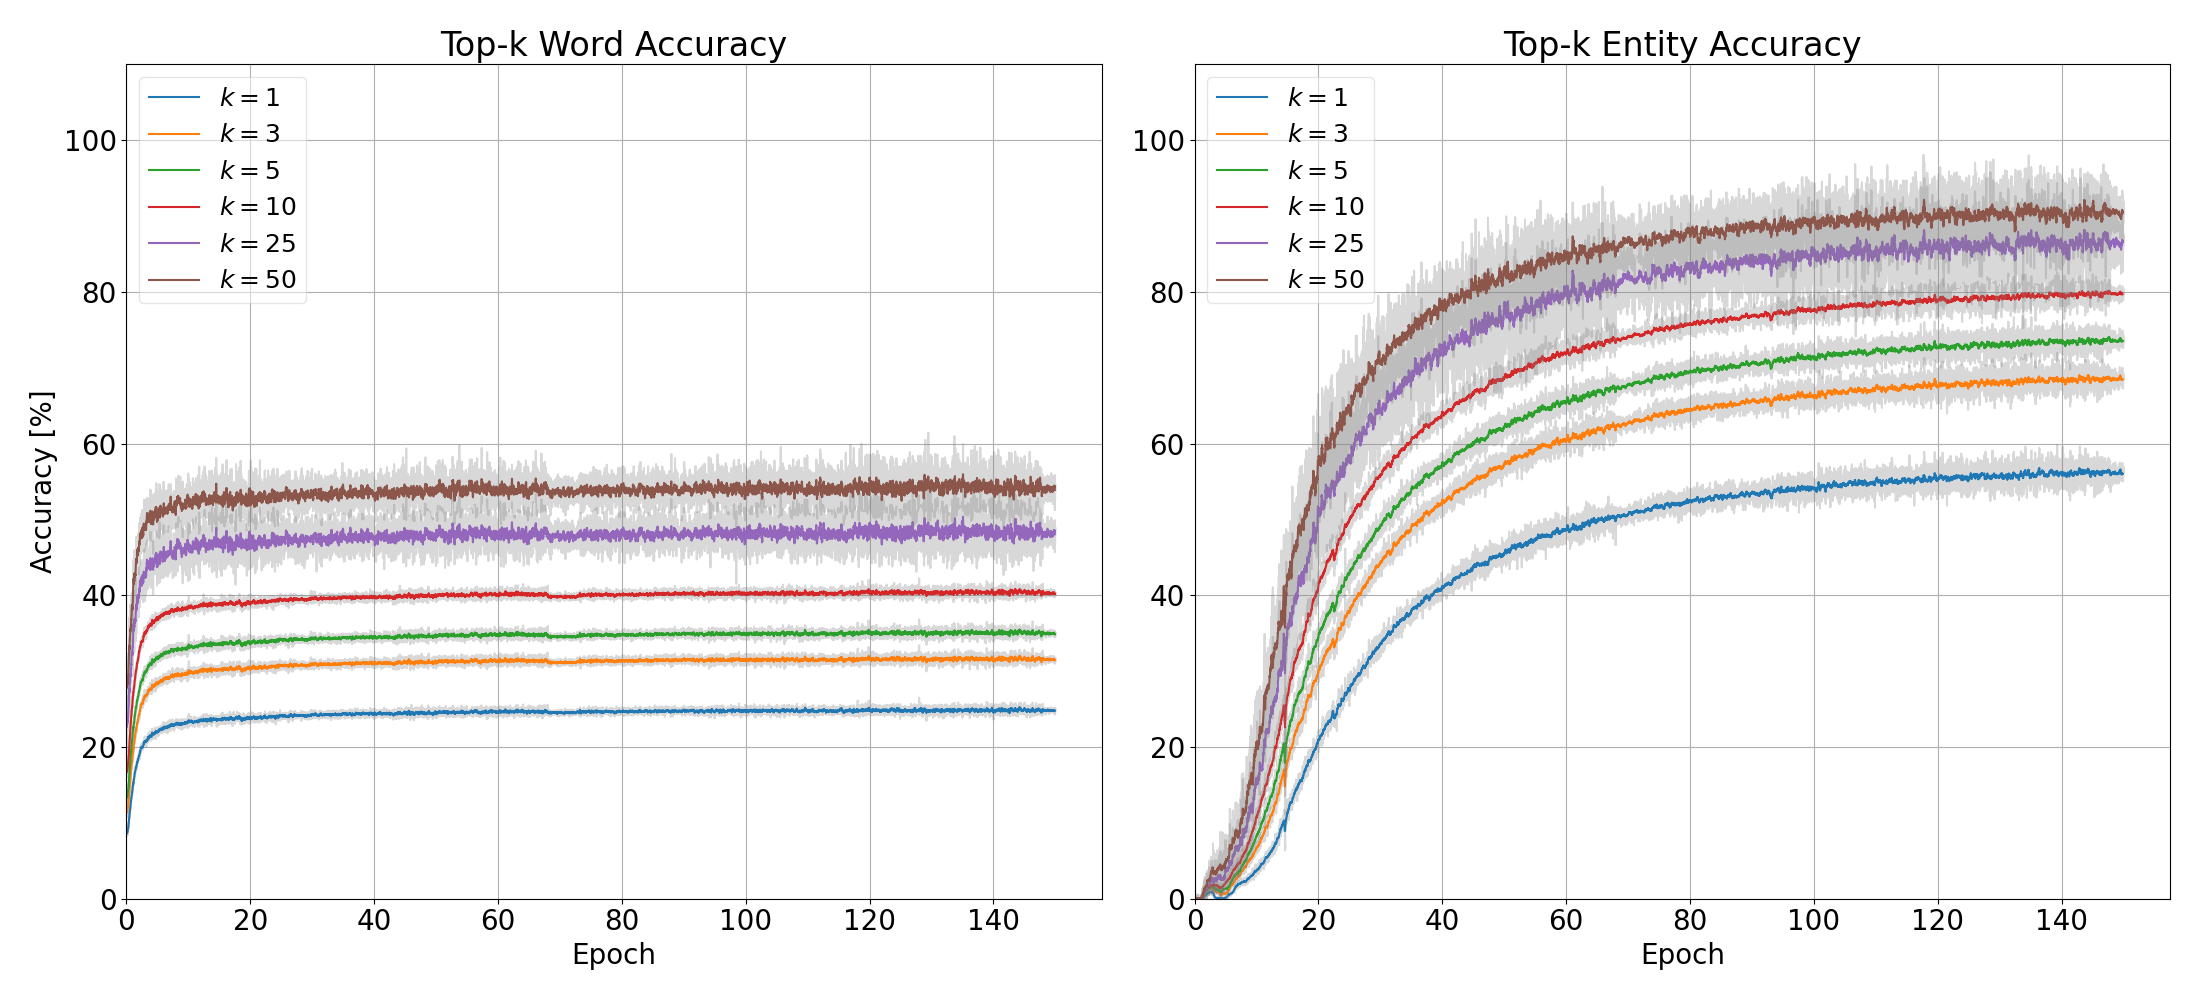
\includegraphics[width=0.8\textwidth]{pretrain-acc}
    \caption{Masked sub-words and masked entity accuracy throughout pretraining.}
    \label{fig:pretrain-acc}
\end{figure}\noindent

\section{Danish Named Entity Recognition}%
\subsection{Main Benchmark: Our Results and Reproduction}

              % precision    recall  f1-score   support

 % ┆   ┆   LOC     0.8365    0.9062    0.8700        96
 % ┆   ┆  MISC     0.7652    0.7273    0.7458       121
 % ┆   ┆   ORG     0.7956    0.6770    0.7315       161
 % ┆   ┆   PER     0.9441    0.9389    0.9415       180

 % ┆ micro avg     0.8467    0.8118    0.8289       558
 % ┆ macro avg     0.8354    0.8124    0.8222       558
% weighted avg     0.8440    0.8118    0.8262       558

              % precision    recall  f1-score   support

 % ┆   ┆   LOC     0.8365    0.9062    0.8700        96
 % ┆   ┆   ORG     0.7956    0.6770    0.7315       161
 % ┆   ┆   PER     0.9441    0.9389    0.9415       180

 % ┆ micro avg     0.8690    0.8352    0.8518       437
 % ┆ macro avg     0.8588    0.8407    0.8477       437
% weighted avg     0.8658    0.8352    0.8484       437
\begin{table}[H]
        \footnotesize
        \begin{center}
                \begin{tabular}{l l | c c c c | c c c c}
                    \multirow{2}{*}{Model name} & \multirow{2}{*}{Trained on} & \multicolumn{4}{c|}{Micro Avg. [\pro]} & \multicolumn{4}{c}{Class F1 [\pro]}\\
                            &  & F1 & F1 {\tiny\textdiscount MISC} & Prec. & Rec. & LOC & PER & ORG & MISC \\
                        \hline
                    DaLUKE & DaNE & 82.89 & 85.18 & 84.67 & 81.18 & \textbf{87.00} & \textbf{94.15} & 73.15 & 74.58 \\\hline
                        DaNLP da-BERT & DaNE & -- & 84.04 & 86.27 & 64.16 & 83.90 & 92.82 & 72.98 & -- \\
                        NERDA m-BERT & DaNE & 79.22 & 81.71 & 82.12 & 76.52 & 83.50 & 92.61 & 66.90 & 70.34 \\
                        NERDA Ælæctra & DaNE & 70.58 & 74.54 & 76.14 & 65.77 & 77.32 & 86.93 & 56.18 & 56.39 \\
                        DaCy medium & DaNE & 78.32 & 80.50 & 78.32 & 78.32 & 83.96 & 90.41 & 66.23 & 70.09 \\
                        DaCy large & DaNE & \textbf{84.91} & \textbf{86.89} & 86.16 & \textbf{83.69} & 85.29 & \textbf{94.15} & \textbf{79.04} & \textbf{78.05} \\
                        DaNLP spaCy & DaNE & 73.75 & 75.73 & 76.15 & 71.51 & 75.96 & 87.87 & 59.57 & 66.06 \\
                        DaNLP Flair & DaNE & -- & 81.78 & \textbf{89.19} & 59.14 & 84.82 & 93.15 & 62.95 & -- \\
                        Polyglot & Wikipedia & -- & 64.18 & 70.30 & 46.24 & 64.95 & 78.74 & 39.30 & -- \\
                        daner & ITU CDT & -- & 56.52 & 64.79 & 39.25 & 59.49 & 70.40 & 28.29 & -- \\
                \end{tabular}
        \end{center}
        \caption{F1\pro-scores of Danish NER models of the DaNE testing dataset consisting of 565 sentences.}
        \label{tab:DaNE}
\end{table}
\subsection{Additional Datasets}
              % precision    recall  f1-score   support

 % ┆   ┆   LOC     0.8298    0.8041    0.8168        97
 % ┆   ┆  MISC     0.0849    0.3000    0.1324        30
 % ┆   ┆   ORG     0.4710    0.6915    0.5603        94
 % ┆   ┆   PER     0.8994    0.9527    0.9253       169

 % ┆ micro avg     0.6054    0.8026    0.6902       390
 % ┆ macro avg     0.5713    0.6871    0.6087       390
% weighted avg     0.7162    0.8026    0.7493       390
              % precision    recall  f1-score   support

 % ┆   ┆   LOC     0.8298    0.8041    0.8168        97
 % ┆   ┆   ORG     0.4710    0.6915    0.5603        94
 % ┆   ┆   PER     0.8994    0.9527    0.9253       169

 % ┆ micro avg     0.7397    0.8444    0.7886       360
 % ┆ macro avg     0.7334    0.8161    0.7675       360
% weighted avg     0.7688    0.8444    0.8008       360
\begin{table}[H]
        \footnotesize
        \begin{center}
                \begin{tabular}{l l | c c c c | c c c c}
                    \multirow{2}{*}{Model name} & \multirow{2}{*}{Trained on} & \multicolumn{4}{c|}{Micro Avg. [\pro]} & \multicolumn{4}{c}{Class F1 [\pro]}\\
                            &  & F1 & F1 {\tiny\textdiscount MISC} & Prec. & Rec. & LOC & PER & ORG & MISC \\
                        \hline
                    DaLUKE & DaNE & \textbf{69.02} & 78.86 & 60.54 & 80.26 & \textbf{81.68} & \textbf{92.53} & 56.03 & 13.24 \\\hline
                    DaNLP da-BERT & DaNE & -- & 79.23 & 73.98 & 78.72 & 78.64 & 93.45 & \textbf{56.88} & -- \\
                        NERDA m-BERT & DaNE & 66.37 & 76.60 & 58.08 & 77.44 & 76.33 & 92.08 & 52.53 & 12.41 \\
                        NERDA Ælæctra & DaNE & 66.28 & 76.09 & 59.96 & 74.10 & 74.87 & 90.32 & 53.00 & 13.24 \\
                        DaCy medium & DaNE & 65.61 & 75.03 & 55.73 & 79.74 & 76.06 & 92.09 & 48.74 & 12.59 \\
                        DaCy large & DaNE & 68.45 & \textbf{79.02} & 58.86 & \textbf{81.79} & 79.02 & \textbf{92.53} & 58.04 & \textbf{15.48} \\
                        DaNLP spaCy & DaNE & 64.11 & 72.70 & 55.92 & 75.13 & 72.73 & 88.33 & 46.51 & 12.31 \\
                        DaNLP Flair & DaNE & -- & 76.16 & \textbf{75.14} & 71.28 & 80.21 & 94.35 & 36.96 & -- \\
                        Polyglot & Wikipedia & -- & 64.10 & 63.49 & 59.74 & 69.74 & 78.38 & 24.69 & -- \\
                        daner & ITU CDT & -- & 59.89 & 61.83 & 53.59 & 58.16 & 73.63 & 26.09 & -- \\
                \end{tabular}
        \end{center}
        \caption{F1\pro-scores of Danish NER models of the Plank testing dataset consisting of 565 sentences.}
        \label{tab:Plank}
\end{table}

              % precision    recall  f1-score   support

 % ┆   ┆   LOC     0.7626    0.7085    0.7346      5242
 % ┆   ┆   ORG     0.6497    0.3347    0.4418      4078
 % ┆   ┆   PER     0.7239    0.7757    0.7489      4378

 % ┆ micro avg     0.7267    0.6187    0.6684     13698
 % ┆ macro avg     0.7121    0.6063    0.6418     13698
% weighted avg     0.7166    0.6187    0.6520     13698
\begin{table}[H]
        \footnotesize
        \begin{center}
                \begin{tabular}{l l | c c c | c c c }
                    \multirow{2}{*}{Model name} & \multirow{2}{*}{Trained on} & \multicolumn{3}{c|}{Micro Avg. [\pro]} & \multicolumn{3}{c}{Class F1 [\pro]}\\
                        & & F1 & Prec. & Rec. & LOC & PER & ORG \\
                        \hline
                    DaLUKE & DaNE & \textbf{66.84} & \textbf{72.67} & 61.87 & 73.46 & 74.89 & 44.18 \\\hline
                        DaNLP da-BERT & DaNE & 65.66 & 68.37 & 63.16 & 72.08 & 74.49 & 40.05 \\
                        NERDA m-BERT & DaNE & 63.40 & 61.28 & 65.68 & 70.72 & 76.87 & 48.35 \\
                        NERDA Ælæctra & DaNE & 48.65 & 48.32 & 48.99 & 56.63 & 69.89 & 24.02 \\
                        DaCy medium & DaNE & 60.05 & 58.37 & 61.84 & 70.71 & 73.74 & 39.27 \\
                        DaCy large & DaNE & 64.55 & 62.18 & \textbf{67.11} & \textbf{74.11} & \textbf{77.18} & \textbf{49.78} \\
                        DaNLP spaCy & DaNE & 59.55 & 58.52 & 60.61 & 68.68 & 71.63 & 38.76 \\
                        DaNLP Flair & DaNE & 65.04 & 70.74 & 60.19 & 70.08 & 74.36 & 43.67 \\
                        Polyglot & Wikipedia & 61.99 & 66.34 & 58.18 & 72.45 & 69.15 & 35.33 \\
                        daner & ITU CDT & 46.59 & 51.54 & 42.51 & 56.15 & 54.51 & 14.76 \\
                \end{tabular}
        \end{center}
        \caption{F1\pro-scores of Danish NER models of the WikiANN testing dataset consisting of 10000 sentences.}
        \label{tab:WikiANN}
\end{table}

\end{document}
